\documentclass{article}

\usepackage{newtxtext,newtxmath}
\usepackage{caption,subcaption}
\usepackage{float}
\usepackage[vmargin=1in, hmargin=1in]{geometry}
\usepackage{graphicx}
\usepackage{listings}
\usepackage{siunitx}
\usepackage{tikz}
\usepackage{xcolor}

\lstdefinestyle{mypy}
{
    language=python,
    basicstyle=\ttfamily,
    commentstyle=\color{green},
    keywordstyle=\color{blue},
    stringstyle=\color{red},
    basewidth={0.5em},
    breakatwhitespace=false,         
    breaklines=true,                 
    captionpos=t,
    frame=single,
    framerule=1pt,
    columns=flexible,                    
    keepspaces=true,
    showspaces=false,
    showstringspaces=false,
    showtabs=false,
    tabsize=4,
}

\lstdefinestyle{mygeo}
{
    language=c++,
    basicstyle=\ttfamily,
    commentstyle=\color{green},
    keywordstyle=\color{blue},
    stringstyle=\color{red},
    basewidth={0.5em},
    breakatwhitespace=false,         
    breaklines=true,                 
    captionpos=t,
    frame=single,
    framerule=1pt,
    columns=flexible,                    
    keepspaces=true,
    showspaces=false,
    showstringspaces=false,
    showtabs=false,
    tabsize=4,
}

\newcommand{\vect}[1]{\ensuremath{\boldsymbol{\mathbf{#1}}}}

\begin{document}

\begin{center}
    {\Large AE708 assignment 2}\\[0.5em]
    {\large 184104002, Potluri Vachan Deep}\\[0.5em]
    {\today}
    \rule{\linewidth}{2pt}
\end{center}

\section*{Notes}
Points 2-4 are taken from slide 20 of the file \texttt{Rocket\_Performance\_Parameters\_Nozzles.pdf}.
\begin{enumerate}
    \item Simulations are performed using OpenFOAM-v9.
    \item All nozzles use throat radius $R_t = \SI{1}{\meter}$ and a converging section as a \SI{75}{\degree} arc of radius $1.5 R_t$.
    \item All nozzles use $\varepsilon = 4 = (R_e/R_t)^2$.
    \item Just after the throat, all nozzles have an arc of angle $\theta_n$ and radius $0.4 R_t$. For Rao nozzle(s), $\theta_n = \SI{30}{\degree}$ while $\theta_n = \SI{15}{\degree}$ for conical nozzle.
    \item Conical nozzle uses a half-cone angle of \SI{15}{\degree}.
    \item Two Rao nozzles are considered with the diverging section length 60\% ($K=0.6$) and 80\% ($K=0.8$) of the conical nozzle.
    \item All geometries are \SI{3}{\degree} bodies of revolution. Axisymmetric simulations are done in OpenFOAM.
    \item Stagnation conditions: $p_0 = \SI{287}{\pascal}$, $T_0 = \SI{1}{\kelvin}$ and $\rho_0 = \SI{1}{\kg\per\meter\cubed}$.
    \item Initial conditions: discontinuity at throat with stagnation conditions imposed on left, and design pressure and temperature on right (without velocity).
    \item Boundary conditions
    \begin{itemize}
        \item Inlet: \texttt{totalPressure} for $p$, \texttt{totalTemperature} for $T$, \texttt{zeroGradient} for $\vect{U}$.
        \item Outlet
        \begin{itemize}
            \item Design condition: \texttt{zeroGradient} for $p,\ T$ and $\vect{U}$.
            \item Off design: \texttt{fixedValue} for $p$, \texttt{zeroGradient} for $T$ and $\vect{U}$.
        \end{itemize}
        \item Wall: \texttt{zeroGradient} for $p$ and $T$, \texttt{slip} for $\vect{U}$.
        \item Azimuthal faces: \texttt{wedge} for $p,\ T$ and $\vect{U}$.
    \end{itemize}
\end{enumerate}

\lstinputlisting[
    style=mypy,
    caption={Python code for designing Rao nozzle}
]{design_rao_nozzle.py}
\lstinputlisting[
    style=mygeo,
    caption={Gmsh code for generating Rao nozzle mesh}
]{rao_mesh2.geo}
\lstinputlisting[
    style=mygeo,
    caption={Gmsh code for generating Conical nozzle mesh}
]{conical_mesh.geo}

\begin{figure}[htb]
    \centering
    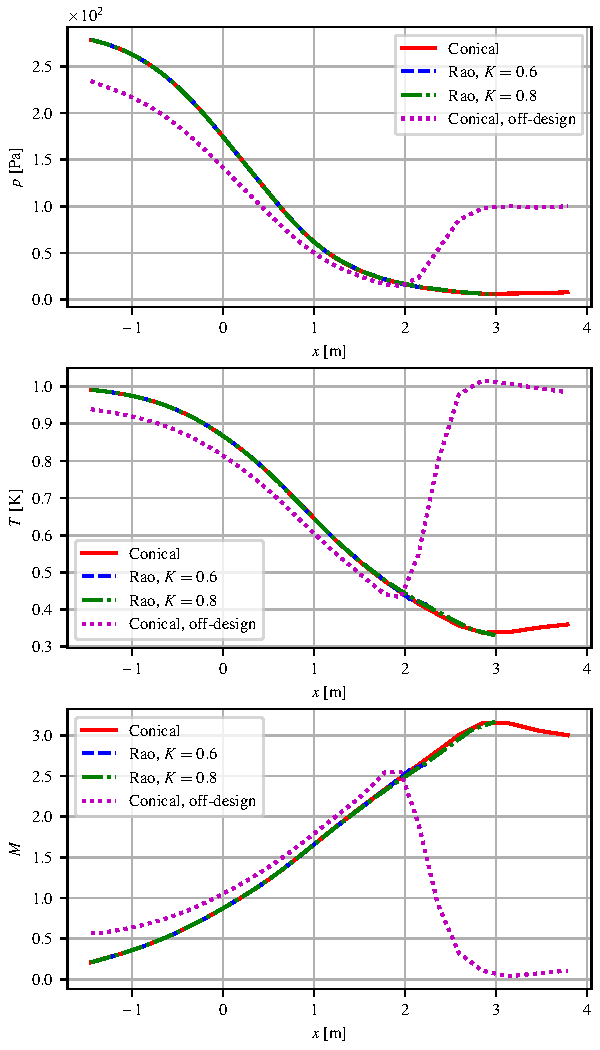
\includegraphics[scale=1]{../plots/pTM_vs_x.pdf}
    \caption{Pressure, Temperature and Mach number variation along the nozzle.}
\end{figure}

\begin{figure}[htb]
    \centering
    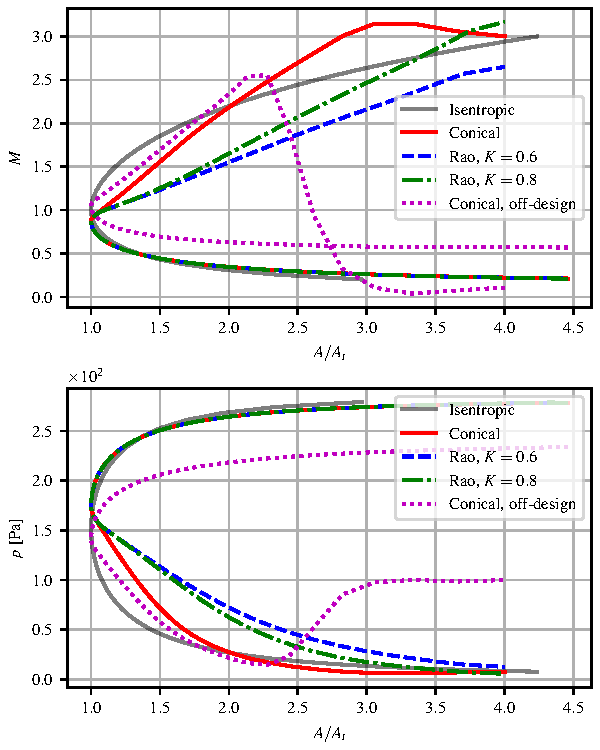
\includegraphics[scale=1]{../plots/Mp_vs_area_ratio.pdf}
    \caption{Mach number and pressure variation with the area ratio.}
\end{figure}

\begin{figure}[htb]
    \def\subfigheight{0.12\textheight}
    \foreach \case/\cptn in {conical/Conical, rao2_K0.6/{Rao, $K=0.6$}, rao2_K0.8/{Rao, $K=0.8$}} {%
        \begin{subfigure}{0.32\linewidth}
            \centering
            \includegraphics[height=\subfigheight]{../run/\case/plots/p_surface_M_contour}
            \caption{\cptn}
        \end{subfigure}
    }
    \caption{Pressure surface plot with \num{30} Mach number contours. Clearly, the Mach number contours are not radial and there is significant multidimensional nature to the flow. Quasi-1D analysis will fail here.}
\end{figure}

\end{document}